\documentclass[letter,12pt]{article}
\usepackage{graphicx}
\usepackage{url}
\usepackage{setspace}
\usepackage{ragged2e}
\usepackage{hanging}
\usepackage{hyperref}
\usepackage{fancyhdr}
\usepackage{lipsum}
\usepackage[none]{hyphenat}
\usepackage{enumitem}
\usepackage{amsmath}

\makeatletter
\newcommand{\distas}[1]{\mathbin{\overset{#1}{\kern\z@\sim}}}
\newsavebox{\mybox}\newsavebox{\mysim}
\newcommand{\distras}[1]{%
	\savebox{\mybox}{\hbox{\kern3pt$\scriptstyle#1$\kern3pt}}%
	\savebox{\mysim}{\hbox{$\sim$}}%
	\mathbin{\overset{#1}{\kern\z@\resizebox{\wd\mybox}{\ht\mysim}{$\sim$}}}%
}
\makeatother

\fancyhead{}
\fancyhead[L]{DISC THROW VARIANCE}
\fancyhead[R]{\thepage}
\fancyfoot{}
\fancypagestyle{plain}{
	\fancyhead{}
	\fancyhead[L]{Running head: DISC THROW VARIANCE}
	\fancyfoot{}
	\fancyhead[R]{\thepage}
}
\pagestyle{fancy}
\renewcommand{\headrulewidth}{0pt}
\addtolength{\headwidth}{\marginparsep}
\addtolength{\headwidth}{\marginparwidth}

\doublespacing

\addtolength{\oddsidemargin}{-.5in}
\addtolength{\evensidemargin}{-.5in}
\addtolength{\textwidth}{1in}

\addtolength{\topmargin}{-.875in}
\addtolength{\textheight}{1.75in}

\begin{document}
	\thispagestyle{plain}
	\begin{center}
		\vspace*{150pt}
		Evaluating Variance in Distance of Disc Throws by Throw Type and Disc Type. \\
		Joshua Katz \& Sejin Kim \\
		Kenyon College \\
	\end{center}
	\vspace*{120pt}
	\centering{Author Note} \\
	\begin{raggedright}
		Joshua Katz \& Sejin Kim, Kenyon College. \\
		Contact: \href{mailto:katz1@kenyon.edu}{katz1@kenyon.edu}, \href{mailto:kim3@kenyon.edu}{kim3@kenyon.edu} \\
		\vspace*{40pt}
		\textit{Keywords:} analysis of variance, ANOVA, frisbee, disc throwing
	\end{raggedright}
	
	\newpage

	\begin{center}
		Evaluating Variance in Distance of Disc Throws by Throw Type and Disc Type.
	\end{center}
	\begin{center}
		\textbf{I. Introduction}
	\end{center}
	\justify
	%PUT THE TEXT HERE, THIS LIPSUM IS FOR SOME FILLER
	This project was inspired by a curiosity that Josh had: is there a statistically significant difference in the distance that a frisbee would fly, depending on how you threw it? It seems obvious: yes, certain types of throws would go further. But, how could this be quantified? The only “hand-wavey” evidence that either of us had seen was the real-world performance in ultimate frisbee games and practices, but throws in a competitive setting aren’t identical. Each throw is thrown in a specific way; some throws are thrown with more or less curve, some are thrown with higher or lower trajectories, and some are specifically thrown to a spot on the field, instead of a player. However, to best measure distance depending on throw type, we need to have data on discs thrown as hard as possible in a straight line. Additionally, there are different types of discs, too. Disc golf discs are shaped differently, and thus have different flight patterns. Would some significant variance arise from this? Because of this, our group was interested in exploring the variance between the three main types of throws, and between two types of discs. \par
	We wanted to evaluate the throw distance of different types of throwing discs using two factors:  the type of disc, a disc golf disc (a “disc”), and a standard USA Ultimate frisbee (a “Frisbee”), and the throw type, backhand, flick, and hammer.  Instead of only measuring the vertical displacement, we also thought that certain throws may have an appreciable amount of horizontal displacement. Therefore, we measured each throw in two-dimensional Euclidean Distance, taking into account horizontal displacement as well as vertical distance. Total distance was measured in meters, and do not need normalized, since all measures will be done from the same scale. We expect the data to be roughly normal, if not skewed slightly higher. All throws will be done in approximately the same environmental conditions to minimize unnecessary noise. \par

	\begin{center}
		\textbf{II. Materials and Procedures}
	\end{center}
	\justify
	In order to explore any variation that might exist, we designed an experiment to find, approximately speaking, the flight distance patterns of the different discs based on the throws. The raw dataset is published as a comma-separated-values spreadsheet on our Github repository. That dataset includes 30 observations of two-dimensional Euclidean distance and the component X and Y distances. Each observation is also marked with the appropriate disc type and throw type. Based on the nature of the data, we decided that no data normalization was needed; that is, we could use the original scale of the data, measured in meters, rather than having to convert the data to a scale of, say, 100. For our main analysis, we will use a two-dimensional Euclidean distance, rounded to the nearest thousandth.\par
  The materials used in the study were a standard USA Ultimate 175 g frisbee, a 172 g Vibram Ridge disc golf putter, and an over-enthusiastic student as the thrower.  In ideal circumstances, we would have used an automated throwing machine to ensure that every throw is released in an optimal manner. Unfortunately, such a machine was not available to us, so instead Josh was tasked with throwing each disc and Frisbee. To account for exhaustion or other effects due to repeated throwing, each throw was determined by a random number generator, using the R script \verb|sample(1:30)|, and assigning each throw a unique ID.\par
  We performed the experiment on McBride Field to take advantage of the yard line markings for vertical (Y) distance, and measured the horizontal (X) displacement by hand. On the day of testing, the weather was clear, with little to no wind effects.there was minimal wind and minimal fluctuations in temperature, humidity, or wind conditions. Each throw was released from the center of the goal line in the south endzone, thrown as far as possible, and as straight ahead as possible. We were only interested in where each throw landed, not where it rolled to. After each throw landed, its vertical distance was measured according to the yard line markings on the field. The horizontal displacement was measured using a one meter long piece of rope, from one of three “anchor” points, which were the center of the field and the hash marks, located seven meters from the center in either direction.\par

	\begin{center}
		\textbf{III. Analysis}
	\end{center}
	\justify
	All of the statistical analysis was done using R, and using the front-end RStudio. In addition to the functions in base R, we also used functions in the \verb|mosaic|, \verb|pwr|, \verb|agricolae|, \verb|multicomp|, and \verb|car| packages. We ran several different tests for analyses of variance, in order to find the differences between the different discs and the different throw types.\par
	
	\begin{center}
		\textbf{a. Exploring the data graphically}
	\end{center}
	\justify
	To determine if there is possibly a significant difference in the standard deviations or the means of the different throws, we created two boxplots to visualize the median distances between different types of discs and different throw types. For disc type, variance in both discs look similar, but there does appear to be a difference in means. When looking at the throwtypes, we can see that the distribution and medians of both the flick and the backhand are comparable, but there is a stark difference between these two throws and the hammer throw.\par
  \begin{center}
    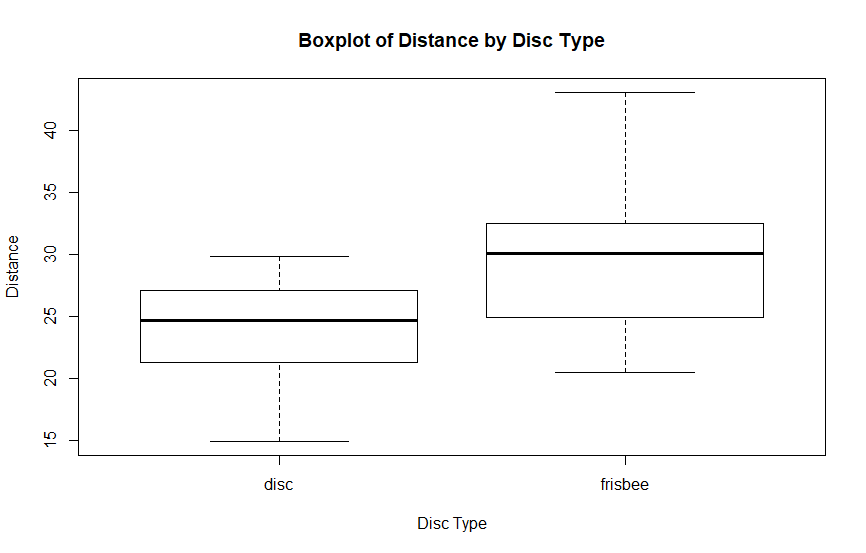
\includegraphics[width=0.8\textwidth]{boxplotdistdisc.png}
    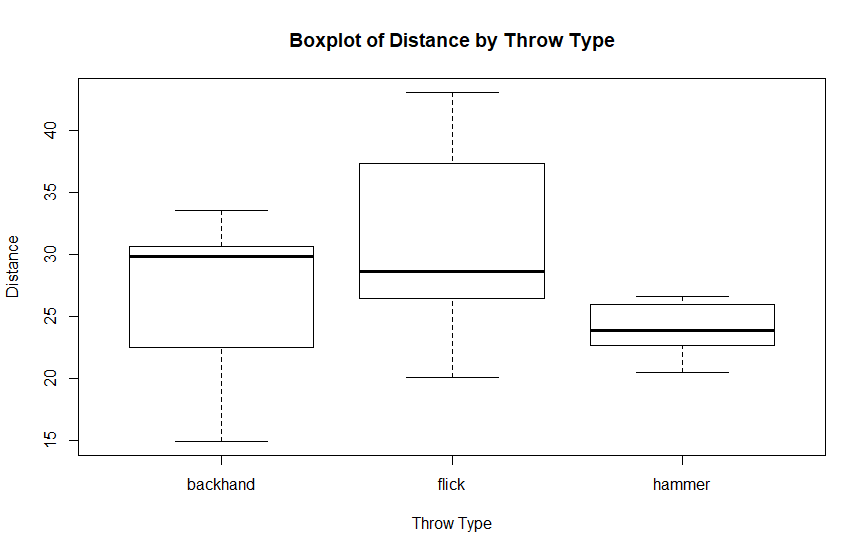
\includegraphics[width=0.8\textwidth]{boxplotdiststhrow.png}
  \end{center}
  We also created a diagnostic plot to see if the tight standard deviations of the hammer could be resolved by using any sort of transformation, and as we will see in part III.c, resolve some of the normality woes as well. In this plot, we can see that the slope of the line is roughly one, with the points falling somewhat close to the line. To find this exactly, we constructed a linear model from the log of the group means and the log of the group standard deviations. The slope of the line turns out to be $\approx 0.03$. This was not as close to 0 as we would have liked it to be, so we attempted to apply some transformations anyways, including a square-root transformation, a logarithmic transformation, and an exponentiation transformation at several different powers. Nonetheless, our original, untransformed data showed the best linearity. Based on this plot and the figures from the diagnostic, we chose to not apply any transformations for our analysis of variance.\par
  \begin{center}
    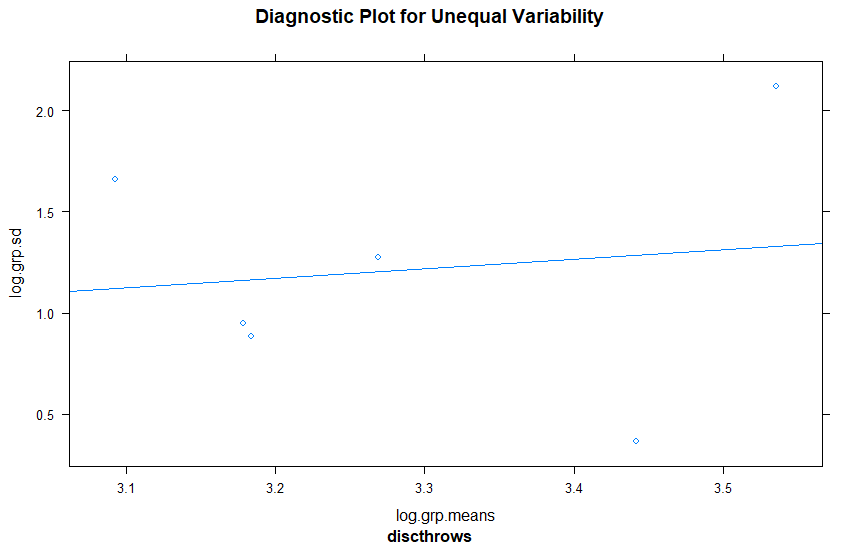
\includegraphics[width=0.8\textwidth]{diagplot.png}
  \end{center}
	
	\begin{center}
		\textbf{b. Analysis of variance}
	\end{center}
	\justify
	Given the findings in the exploratory data analysis above, we chose to run a two-way analysis of variance to compare the variance between the different types of discs and the different types of throws. We were interested in the interaction between the throw type and the disc type. We suspected that certain discs may impact the distance, based on the throw type. For example, we might have seen that, because a disc golf disc is not designed to be thrown using the hammer, we would see dramatically decreased performance from that disc when thrown using the hammer. An inverse effect might also be present, where a certain disc performs exceptionally well using a certain throw type, or vice versa.\par
  We started by generating an interaction plot, using the \verb!interaction.plot()! function. These plots are shown below. In the plots shown below, we can see that there is a possible interaction effect. Of note is, in the interaction plot for distance by disc type, we found that while flick and backhand lines are close enough to parallel for us to rule out interaction, these two slopes were visibly different from the slope of the line for hammer throws. In this plot, we can actually see that the line for the backhand throw and the hammer intersect, indicating a strong possibility of an interaction effect. The same is reflected in the interaction plot for distance by throw type, where the difference in slopes between the frisbee and the disc appear to be roughly equal between backhand and flicks, but visibly different between flicks and hammers.\par
  \begin{center}
    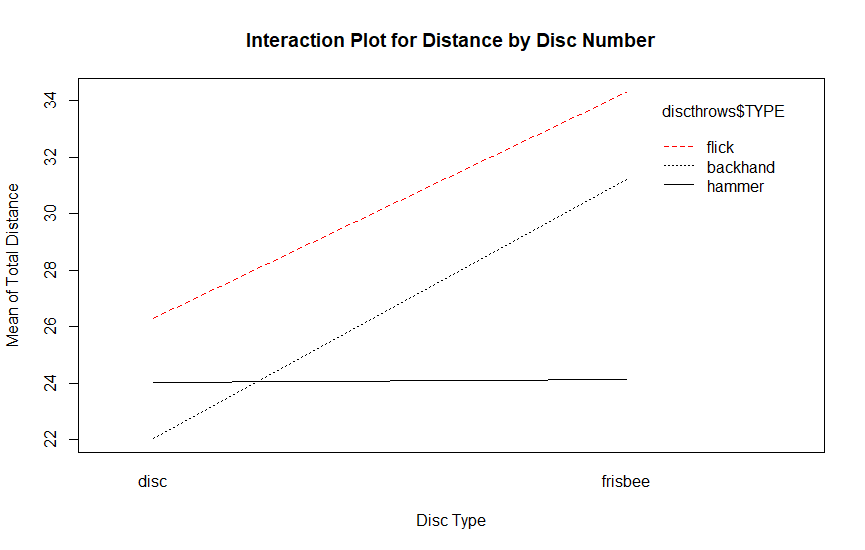
\includegraphics[width=0.8\textwidth]{intdistdisc.png}
    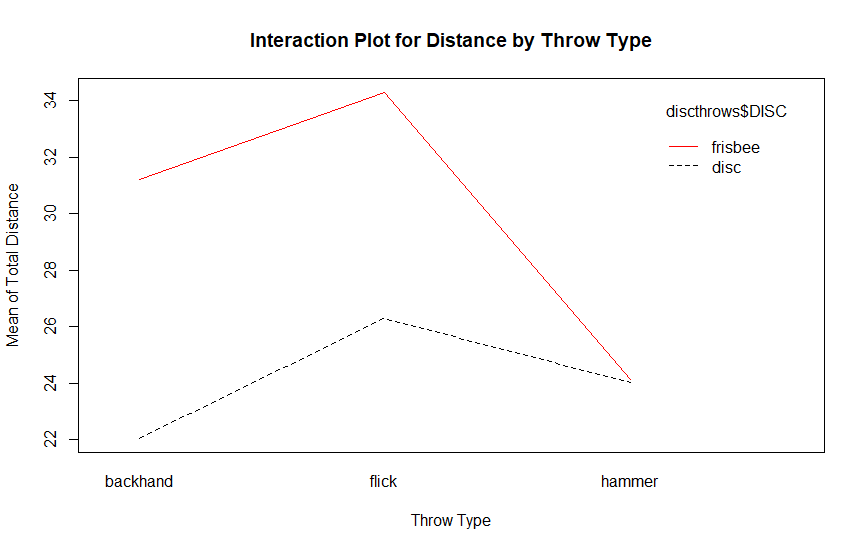
\includegraphics[width=0.8\textwidth]{interactiondistthrow.png}
  \end{center}
  Based on these plots, we saw it fit to run an interaction analysis, by generating a two way ANOVA table with interaction, using the disc type, the throw type, and the interaction between the disc and throw types. After running the interaction analysis, we found that the interaction effect was not significant with a $F$-value of 2.649 on 2 degrees of freedom and a $p$-value of $0.09 > 0.05 = \alpha$. Given this, we decided that any interaction effect would not be significant. The interaction term between disc type and throw type has been dropped from any further analysis.\par
  We began our analysis by conducting an overall F-test for the model. To do this, we created an analysis of variance table on the total distance by the disc type and throw type, or the full model. We also created an analysis of variance table of total distance alone, or the null model. We then ran an analysis of variance on the full model against the null model. We found that the overall variance has a F-statistic of 5.3822 on (24, 29) residual degrees of freedom, and a $p$-value of 0.00186. By this, we can conclude that some difference exists between the different factors.\par
  We then ran a F-test for two-way interactions, using \textit{distance} as the response variable, being predicted by \textit{disc} and \textit{type}. In this, we found that the difference in means of the different disc types was statistically significant, with a F-statistic of 12.095 on one degree of freedom, and a $p$-value of $0.00195 < 0.05 = \alpha$. We also found that the difference in means of the different throw types was statistically significant, with a F-statistic of 4.759 on two degrees of freedom, and a $p$-value of $0.01817 < 0.05 = \alpha$. Like we stated above, we found that the interaction term was not significant at a $\alpha = 0.05$ significance level.\par
  We continued by conducting a F-test for each main effect: disc type and throw type. To do this, we ran Fisher’s least significant difference (“LSD”) test for both disc and throw type. We used no method for adjusting the $p$-values, and we computed the LSD using the analysis of variance table that was used for the F-test for two-way interactions. We then had R group our throw and disc types based on that. We found that there was a statistically significant difference between throwing a flick and a hammer, where flicks are thrown further than hammers. However, there was no difference between backhands and flicks or hammers. We also found that there was a statistically significant difference between using a frisbee and a disc; frisbees are, on average, flew further than discs.\par
	
	\begin{center}
		\textbf{c. Conditions for the ANOVA}
	\end{center}
	\justify
	We chose to run a Levene test to check the condition for equal variance, using the \verb!leveneTest()! function in R. We ran the calculations according to a two-way analysis of variance. In this, we found that with an $F$-value of 1.492 on 5 degrees of freedom, we have a $p$-value of $0.2297 > 0.05 = \alpha$. Based on this, we have no statistical evidence to suggest that the equal variance condition is being violated.\par
	This finding is also supported in the residuals versus fitted values plot. In the plot shown below we see that all of the data points are fairly well distributed vertically. Of course, this is not perfect, but there is nothing in particular to worry about; unevenness and imperfectness to be expected in any real-world dataset.\par
	\begin{center}
    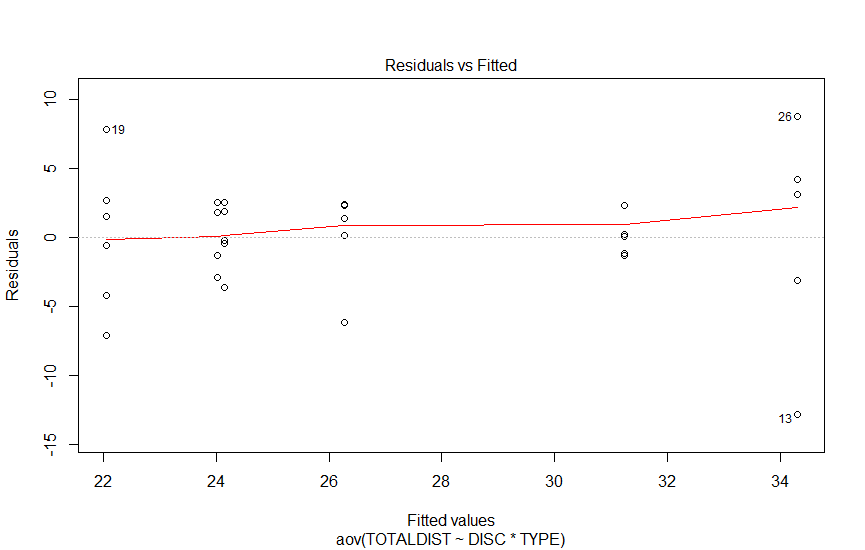
\includegraphics[width=0.8\textwidth]{resfitthrow.png}
  \end{center}
  In our normal quantile-quantile plot, we see that the normality condition for an analysis of variance is not perfect, but some uncertainty is to be expected. It is worth noting that tails of the plot looks like it could possibly be fixed by a transformation, but as we tried in section III.a, we could not find an appropriate transformation. We feel comfortable with the level of normality that is presented in this plot.\par
  \begin{center}
    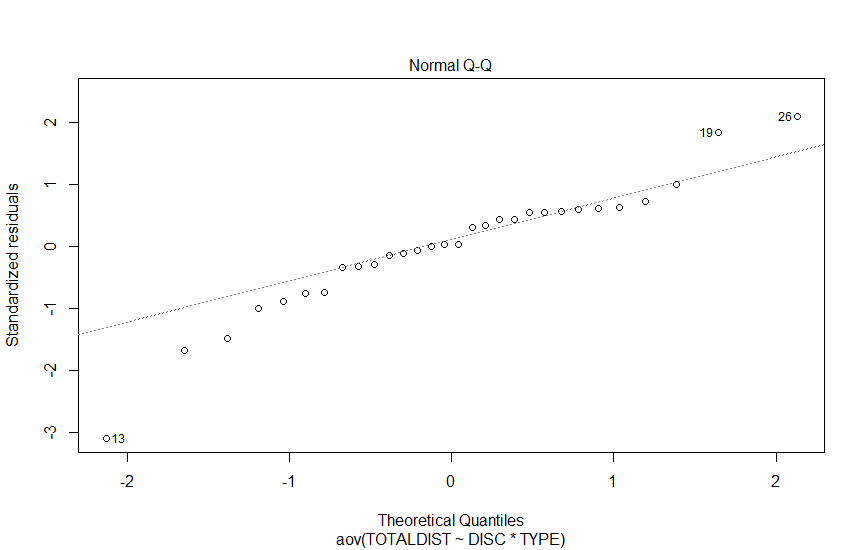
\includegraphics[width=0.8\textwidth]{normalthrow.png}
  \end{center}
  We are confident that our testing methodology and experimental design have satisfied the zero-mean residual condition and the independence condition.\par
	
	\begin{center}
		\textbf{IV. Results and the Model}
	\end{center}
	\justify
	Given the above model-building procedures and F-tests, we chose to use the two-way ANOVA model with an interaction term,
	$$Y_{ij} = \mu + \tau_{i} + \beta_{j} + \gamma_{ij} + \epsilon_{ijk}$$
	for $i = 1, 2$, $j = 1, 2, 3$, and $k=1, 2, 3, 4, 5$. In this model, $\tau_{i}$ represents the effect due to the $i$-th level of the disc type, $\beta_{j}$ represents the effect due to the $j$-th level of the throw type, and $\gamma_{ij}$ represents the effect due to any effect between the $i$-th of disc type and $j$-th level of throw type. Because disc type and throw type are predetermined, categorical variables, we are using a fixed-effects model for this analysis.\par
	As we have shown above, the interaction effect between disc type and throw type is not significant, with a $p$-value of $0.091 > 0.05 = \alpha$, with a $F$-statistic of 2.64 on two degrees of freedom. As a result, we decided to not run a Tukey honest significant difference test. \par
	We then used the means of the groups to create groups and range plots, shown below. In this analysis, we found that there was a statistically significant difference between using a flick and a hammer, but there was no significant difference between using a flick or a backhand, or between using a backhand and a hammer. We also found that there was a statistically significant difference of means between frisbee throws and disc throws.\par
	\begin{center}
    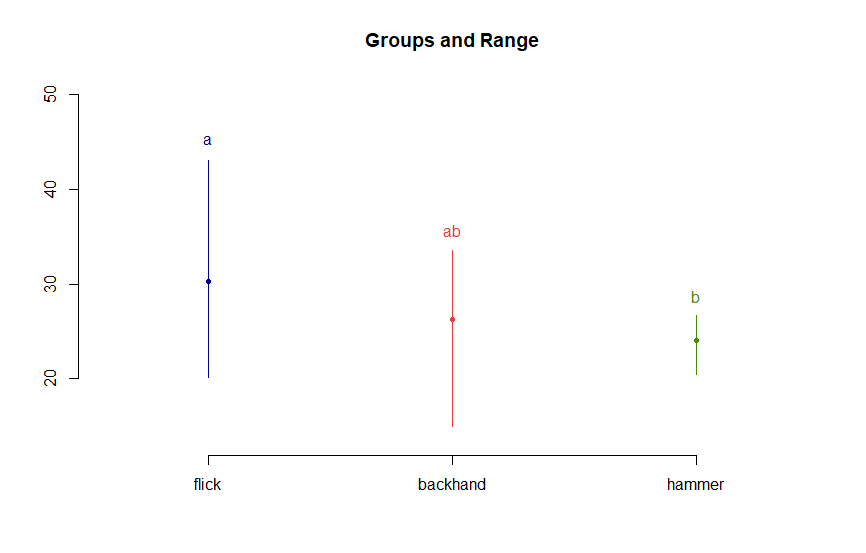
\includegraphics[width=0.8\textwidth]{grouprangethrow.png}
    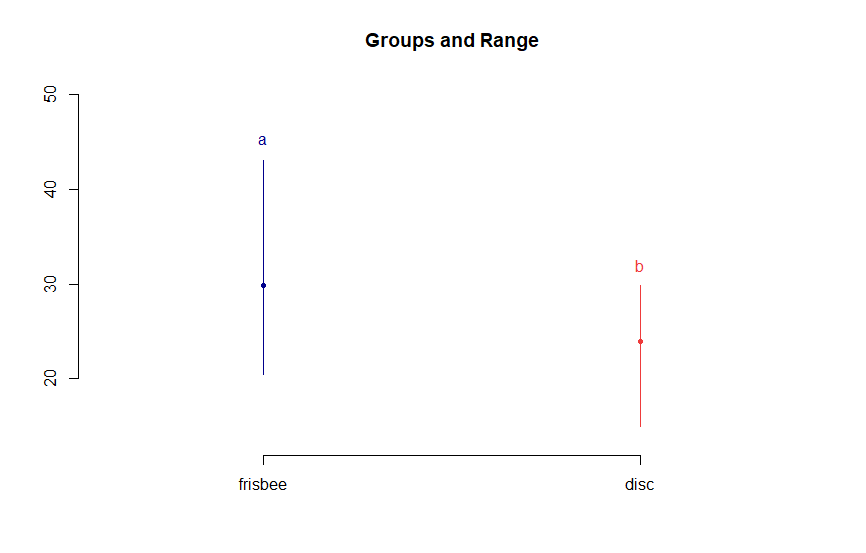
\includegraphics[width=0.8\textwidth]{grouprangedisc.png}
  \end{center}
  Of course, the expansiveness of this study is questionable; the throwing style that Josh used is unique to him. However, we can make the following conclusions. If we are looking to maximize distance, we should use a flick or a backhand throw, and should use a frisbee. There is no statistically significant difference in the means of the flicks and the means of the backhands. If we are looking to minimize distance, we should use a hammer or a backhand throw, and should use a disc. Again, there is no statistically significant difference in the means of the groups.\par
	
	\begin{center}
		\textbf{V. Further Discussion}
	\end{center}
	\justify
	As we discussed earlier, our analysis of the data went on a tangent to investigate horizontal displacement. Specifically, we were curious if disc type or throw type affected the horizontal displacement of a throw. Because this tangent is not central to our paper, it will be briefly summarized instead of presenting another full analysis.\par
	Viewing an interaction plot revealed that there is some sort of interaction present in the data, so we included an interaction term in the model. A cursory glance at some EDA revealed that equal variance across different throw types may not be met, and after viewing the appropriate residual plots, we found that a transformation of the horizontal displacement variable may be necessary for this analysis.\par
	To check what transformation might be appropriate, we created a diagnostic plot for horizontal displacement. The slope was 0.645, so we decided to try two different transformations: a square root transformation (since 0.645 is relatively close to 0.5, and a slope of 0.5 would indicate a square root transformation), and a transformation of horizontal displacement. Both of these transformations fixed the standard deviation issue, but for both transformations, the condition of normally distributed residuals is nowhere close to being met. As such, we decided to continue with our analysis of horizontal displacement using the original data. \par
	After running a two way analysis of variance with interaction, we found that the interaction term was significant, which meant we should run Tukey’s Honest Significant Distance on the means of all possible combinations of throw and disc type to see which combinations had significant differences. The results of this test revealed that there were only two combinations with significant differences.\par
	We encountered several issues while performing our experiment. First, one of the throws was misread, so we threw 6 disc-backhands and 4 disc-hammers, instead of the intended 5 disc-backhands and 5 disc-hammers. While it doesn’t directly affect our results, it should be noted that our data is not balanced.\par
	Additionally, Josh had never thrown a disc prior to performing the experiment, nor is he particularly great at throwing frisbees. If we were to perform this experiment again, we would absolutely ensure that whoever is throwing has had ample experience using both discs and frisbees, and is a strong thrower with both discs and frisbees.\par
	
	\newpage
	
	\begin{center}
		Works Cited
	\end{center}
	\raggedright
	\begin{hangparas}{.5in}{1}
		Felipe de Mendiburu (2019). agricolae: Statistical Procedures for Agricultural Research. R package version 1.3-1. https://CRAN.R-project.org/package=agricolae
	\end{hangparas}
	\begin{hangparas}{.5in}{1}
		John Fox and Sanford Weisberg (2019). An {R} Companion to Applied Regression, Third Edition. Thousand Oaks CA: Sage. URL: https://socialsciences.mcmaster.ca/jfox/Books/Companion/
	\end{hangparas}
	\begin{hangparas}{.5in}{1}
		R Core Team (2019). R: A language and environment for statistical computing. R Foundation for Statistical Computing, Vienna, Austria. URL https://www.R-project.org/.
	\end{hangparas}
	\begin{hangparas}{.5in}{1}
		R. Pruim, D. T. Kaplan and N. J. Horton. The mosaic Package: Helping Students to 'Think with Data' Using R (2017). The R Journal, 9(1):77-102.
	\end{hangparas}
	\begin{hangparas}{.5in}{1}
		Stephane Champely (2018). pwr: Basic Functions for Power Analysis. R package version 1.2-2. https://CRAN.R-project.org/package=pwr
	\end{hangparas}
	\begin{hangparas}{.5in}{1}
		Torsten Hothorn, Frank Bretz and Peter Westfall (2008). Simultaneous Inference in General Parametric Models. Biometrical Journal 50(3), 346--363.
	\end{hangparas}
\end{document}
